\documentclass[12pt]{report}
\usepackage[utf8]{inputenc}
\usepackage[russian]{babel}
%\usepackage[14pt]{extsizes}
\usepackage{listings}

\usepackage{graphicx}
\graphicspath{{src/}}
\DeclareGraphicsExtensions{.pdf,.png,.jpg}

\usepackage{amsmath,amsfonts,amssymb,amsthm} 

% Для листинга кода:
\lstset{ %
language=c++,                 % выбор языка для подсветки (здесь это С++)
basicstyle=\small\sffamily, % размер и начертание шрифта для подсветки кода
numbers=left,               % где поставить нумерацию строк (слева\справа)
numberstyle=\tiny,           % размер шрифта для номеров строк
stepnumber=1,                   % размер шага между двумя номерами строк
numbersep=5pt,                % как далеко отстоят номера строк от подсвечиваемого кода
showspaces=false,            % показывать или нет пробелы специальными отступами
showstringspaces=false,      % показывать или нет пробелы в строках
showtabs=false,             % показывать или нет табуляцию в строках
frame=single,              % рисовать рамку вокруг кода
tabsize=2,                 % размер табуляции по умолчанию равен 2 пробелам
captionpos=t,              % позиция заголовка вверху [t] или внизу [b] 
breaklines=true,           % автоматически переносить строки (да\нет)
breakatwhitespace=false, % переносить строки только если есть пробел
escapeinside={\#*}{*)}   % если нужно добавить комментарии в коде
}

% Для измененных титулов глав:
\usepackage{titlesec, blindtext, color} % подключаем нужные пакеты
\definecolor{gray75}{gray}{0.75} % определяем цвет
\newcommand{\hsp}{\hspace{20pt}} % длина линии в 20pt
% titleformat определяет стиль
\titleformat{\chapter}[hang]{\Huge\bfseries}{\thechapter\hsp\textcolor{gray75}{|}\hsp}{0pt}{\Huge\bfseries}


% plot
\usepackage{pgfplots}
\usepackage{filecontents}
\usetikzlibrary{datavisualization}
\usetikzlibrary{datavisualization.formats.functions}


\begin{document}
\begin{titlepage}
	\centering
	{\scshape\LARGE МГТУ им. Баумана \par}
	\vspace{3cm}
	{\scshape\Large Лабораторная работа №4\par}
	\vspace{0.5cm}	
	{\scshape\Large По курсу: "Анализ алгоритмов"\par}
	\vspace{1.5cm}
	{\huge\bfseries Параллельное умножение матриц\par}
	\vspace{2cm}
	\Large Работу выполнила: Оберган Татьяна, ИУ7-55Б\par
	\vspace{0.5cm}
	\LargeПреподаватели:  Волкова Л.Л., Строганов Ю.В.\par

	\vfill
	\large \textit {Москва, 2019} \par
\end{titlepage}

\tableofcontents

\newpage
\chapter*{Введение}
\addcontentsline{toc}{chapter}{Введение}
Цель работы: изучение возможности параллельных вычислений и использование такого подхода на практике. Реализация парралельного алгоритма Винограда умножения матриц. В данной лабораторной работе рассматривается алгоритм Винограда и параллельный алгоритм Винограда. Необходимо сравнить зависимость времени работы алгоритма от числа параллельных потоков и размера матриц, провести сравнение стандартного и параллельного алгоритмов.



\chapter{Аналитическая часть}
Матрицей A размера $[m*n]$ называется прямоугольная таблица
чисел, функций или алгебраических выражений, содержащая m строк и n столбцов. Числа m и n определяют размер матрицы.\cite{Beloysov} Если число столбцов в первой матрице совпадает с числом строк во второй, то эти две матрицы можно перемножить. У произведения будет столько же строк, сколько в первой матрице, и столько же столбцов, сколько во второй.
	    
Пусть даны две прямоугольные матрицы А и В размеров $[m * n]$ и $[n * k]$ соответственно.  
В результате произведение матриц A и B получим матрицу C размера $[m *  k]$.


$c_{i,j} = \sum\limits_{r=1}^n a_{i,r}\cdot b_{r,j}$ называется произведением матриц A и B \cite{Beloysov}.


\section{Алгоритм Винограда}
Подход Алгоритма Винограда является иллюстрацией общей методологии, начатой в 1979-х годах на основе
билинейных и трилинейных форм, благодаря которым большинство усовершенствований для умножения матриц были получены \cite{Gall2012}.

Рассмотрим два вектора $V = (v1, v2, v3, v4)$ и $W = (w1, w2, w3, w4)$.  

 Их скалярное произведение равно (\ref{formula}) 

\begin{equation} \label{formula}
V \cdot W=v_1 \cdot w_1 + v_2 \cdot w_2 + v_3 \cdot w_3 + v_4 \cdot w_4
\end{equation}

Равенство (\ref{formula}) можно переписать в виде(\ref{formula2}) 
\begin{equation} \label{formula2}
V \cdot W=(v_1 + w_2) \cdot (v_2 + w_1) + (v_3 + w_4) \cdot (v_4 + w_3) - v_1 \cdot v_2 - v_3 \cdot v_4 - w_1 \cdot w_2 - w_3 \cdot w_4
\end{equation}

Менее очевидно, что выражение в правой части последнего равенства допускает предварительную обработку: его части можно вычислить заранее и запомнить для каждой строки первой матрицы и для каждого столбца второй. 
Это означает, что над предварительно обработанными элементами нам придется выполнять лишь первые два умножения и последующие пять сложений, а также дополнительно два сложения. 

\subsection{Параллельный алгоритм Винограда}
Трудоемкость алгоритма Винограда имеет сложность $O(nmk)$ для умножения матриц $n1 \times m1$ на $n2 \times m2$. Чтобы улучшить алгоритм, следует распараллелить ту часть алгоритма, которая содержит 3 вложенных цикла.\\

Вычисление результата для каждой строки не зависит от результата выполнения умножения для других строк. Поэтому можно распараллелить часть кода, где происходят эти действия. Каждый поток будет выполнять вычисления определенных строк результирующей матрицы.
	
\section{Параллельное программирование}
	
При использовании многопроцессорных вычислительных систем с общей памятью обычно предполагается, что имеющиеся в составе системы процессоры обладают равной производительностью, являются равноправными при доступе к общей памяти, и время доступа к памяти является одинаковым (при одновременном доступе нескольких процессоров к одному и тому же элементу памяти очередность и синхронизация доступа обеспечивается на аппаратном уровне). Многопроцессорные системы подобного типа обычно именуются симметричными мультипроцессорами (symmetric multiprocessors, SMP).

Перечисленному выше набору предположений удовлетворяют также активно развиваемые в последнее время многоядерные процессоры, в которых каждое ядро представляет практически независимо функциони рующее вычислительное устройство.

Обычный подход при организации вычислений для многопроцессорных вычислительных систем с общей памятью – создание новых параллельных методов на основе обычных последовательных программ, в которых или автоматически компилятором, или непосредственно программистом выделяются участки независимых друг от друга вычислений. Возможности автоматического анализа программ для порождения параллельных вычислений достаточно ограничены, и второй подход является преобладающим. При этом для разработки параллельных программ могут применяться как новые алгоритмические языки, ориентированные на параллельное программирование, так и уже имеющиеся языки, расширенные некоторым набором операторов для параллельных вычислений.

Широко используемый подход состоит и в применении тех или иных библиотек, обеспечивающих определенный программный интерфейс (application programming interface, API) для разработки параллельных программ. В рамках такого подхода наиболее известны Windows Thread API. Однако первый способ применим только для ОС семейства Microsoft Windows, а второй вариант API является достаточно трудоемким для использования и имеет низкоуровневый характер \cite{Barkalov}.

\subsection{Организация взаимодействия параллельных потоков}
Потоки исполняются в общем адресном пространстве параллельной программы. Как результат, взаимодействие параллельных потоков можно организовать через использование общих данных, являющихся доступными для всех потоков. Наиболее простая ситуация состоит в использовании общих данных только для чтения. В случае же, когда общие данные могут изменяться несколькими потоками, необходимы специальные усилия для организации правильного взаимодействия.


\section{Вывод}
Был рассмотрен алгоритм Винограда и возможность его оптимизации с помощью распараллеливания потоков. Была рассмотрена технология параллельного программирования и
организация взаимодействия параллельных потоков.



\chapter{Конструкторская часть}
\textbf{Требования к вводу:}
На вход подаются две матрицы
\newline
\textbf{Требования к программе:}
\begin{itemize}
\item корректное умножение двух матриц;
\item при матрицах неправилыных размеров программа не должна аварийно завершаться.
\end{itemize}

\section{Схемы алгоритмов}
В данной части будет рассмотрена схема алгоритма Винограда (Рис. 2. 1) и выбранный спрособ распараллеливания.

\begin{figure}[!htbp]
\centering
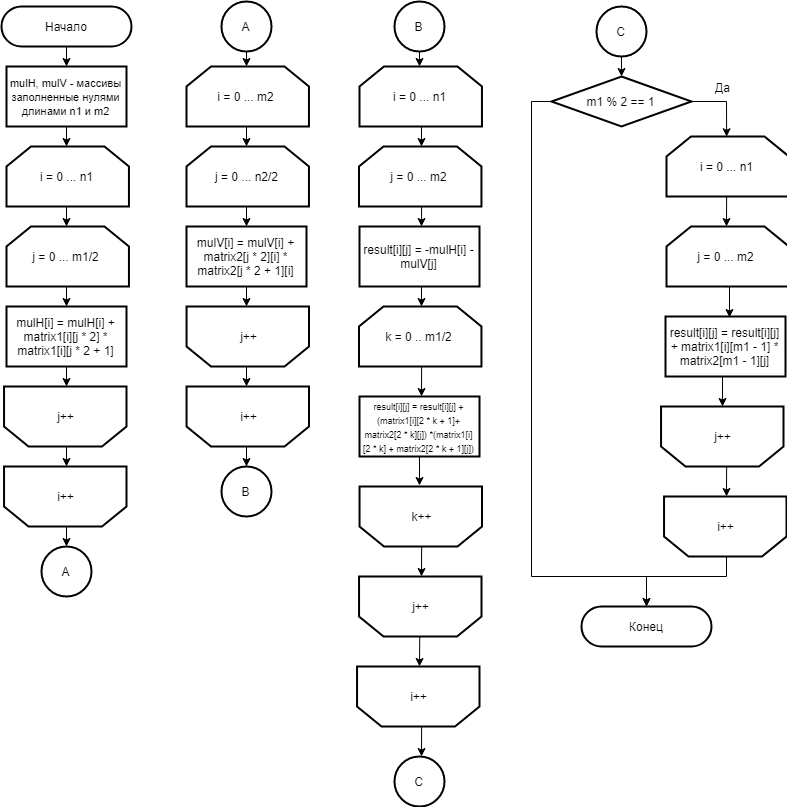
\includegraphics[scale=0.6]{SchemeVin}
\caption{Схема алгоритма Винограда}
\label{fig:mpr}
\end{figure}

\newpage

\section{Распараллеливание программы}
Распрараллеливание программы должно ускорять время работы. Это достигается за счет реализации в узких участках (напимер в циклах с большим количеством независимых вычилений).

В предложенном алгоритме данным участком будет являться тройной цикл поиска результата.
Данный блок программы как раз предлагается распараллелить.
На (Рис. 2.1) это участок между B и С. 

\section{Вывод}
В данном разделе была рассмотрена схема алгоритма Винограда и способ ее распараллеливания.

 

\chapter{Технологическая часть}
Замеры времени были произведены на: Intel(R) Core(TM) i5-8300H, 4 ядра, 8 логических процессоров.

\section{Выбор ЯП}
В качестве языка программирования был выбран C\# \cite{Microsoft} так как этот
язык поддерживает управление потоками на уровне ОС(незеленые потоки). Средой разработки Visual Studio. 
Время работы алгоритмов было замерено с помощью класса Stopwatch. Многопоточное программирование было
реализовано с помощью пространства имен System.Threading.

\section{Сведения о модулях программы}
Программа состоит из:
\begin{itemize}
	\item Program.cs - главный файл программы, в котором располагается точка входа в программу и функция замера времени;
	\item Mult.cs - файл класса Mult, в которм находится обычный алгоритм Винограда;
	\item ParallelMult.cs - файл класса ParallelMult, в котором находится параллельная реализация алгоритма Винограда.
\end{itemize}


\section{Листинг кода алгоритмов}


\begin{lstlisting}[label=some-code,caption=Алгоритм Винограда]
public static int[][] MultVin(int[][] matr1, int[][] matr2)
        {
            int n1 = matr1.Length;
            int n2 = matr2.Length;

            if (n1 == 0 || n2 == 0)
                return null;

            int m1 = matr1[0].Length;
            int m2 = matr2[0].Length;

            if (m1 != n2)
                return null;

            int[] mulH = new int[n1];
            int[] mulV = new int[m2];

            int[][] res = new int[n1][];
            for (int i = 0; i < n1; i++)
                res[i] = new int[m2];

            for (int i = 0; i < n1; i++)
            {
                for (int j = 0; j < m1 / 2; j++)
                {
                    mulH[i] = mulH[i] + matr1[i][j * 2] * matr1[i][j * 2 + 1];
                }
            }

            for (int i = 0; i < m2; i++)
            {
                for (int j = 0; j < n2 / 2; j++)
                {
                    mulV[i] = mulV[i] + matr2[j * 2][i] * matr2[j * 2 + 1][i];
                }
            }

            for (int i = 0; i < n1; i++)
            {
                for (int j = 0; j < m2; j++)
                {
                    res[i][j] = -mulH[i] - mulV[j];
                    for (int k = 0; k < m1 / 2; k++)
                    {
                        res[i][j] = res[i][j] + (matr1[i][2 * k + 1] + matr2[2 * k][j]) * (matr1[i][2 * k] + matr2[2 * k + 1][j]);
                    }
                }
            }

            if (m1 \% 2 == 1)
            {
                for (int i = 0; i < n1; i++)
                {
                    for (int j = 0; j < m2; j++)
                    {
                        res[i][j] = res[i][j] + matr1[i][m1 - 1] * matr2[m1 - 1][j];
                    }
                }
            }

            return res;
        }
\end{lstlisting}


\begin{lstlisting}[label=some-code,caption=Параллельный алгоритм Винограда]
public static int[][] ParallelMultVin(int[][] matr1, int[][] matr2, int nThreads)
        {
            int n1 = matr1.Length;
            int n2 = matr2.Length;

            if (n1 == 0 || n2 == 0)
                return null;

            int m1 = matr1[0].Length;
            int m2 = matr2[0].Length;

            if (m1 != n2)
                return null;

            int[] mulH = new int[n1];
            int[] mulV = new int[m2];

            int[][] res = new int[n1][];
            for (int i = 0; i < n1; i++)
                res[i] = new int[m2];

            Thread[] t = new Thread[nThreads];

            for (int i = 0; i < n1; i++)
            {
                for (int j = 0; j < m1 / 2; j++)
                {
                    mulH[i] = mulH[i] + matr1[i][j * 2] * matr1[i][j * 2 + 1];
                }
            }

            for (int i = 0; i < m2; i++)
            {
                for (int j = 0; j < n2 / 2; j++)
                {
                    mulV[i] = mulV[i] + matr2[j * 2][i] * matr2[j * 2 + 1][i];
                }
            }


            int rowsForThread = n1 / nThreads;
            int n1St = 0;
            for (int i = 0; i < nThreads; i++)
            {
                int n1End = n1St + rowsForThread;
                if (i == nThreads - 1)
                    n1End = n1;
                AllParameters p = new AllParameters(res, matr1, matr2, mulV, mulH, n1St, n1End, m2, m1);

                t[i] = new Thread(MainCycleOptimize);
                t[i].Start(p);

                n1St = n1End;
            }
            foreach (Thread thread in t)
            {
                thread.Join();
            }


            if (m1 \% 2 == 1)
            {
                for (int i = 0; i < n1; i++)
                {
                    for (int j = 0; j < m2; j++)
                    {
                        res[i][j] = res[i][j] + matr1[i][m1 - 1] * matr2[m1 - 1][j];
                    }
                }
            }

            return res;
        }
\end{lstlisting}

\begin{lstlisting}[label=some-code,caption=Распараллеленный главный цикл с оптимизацией адрессации]
        // This addresation works faster
        public static void MainCycleOptimize(object obj)
        {
            AllParameters p = (AllParameters)obj;
            int[][] res = p.res, matr1 = p.matr1, matr2 = p.matr2;
            int[] mulH = p.mulH, mulV = p.mulV;
            int st = p.St, end = p.End;
            int end2 = p.End2, end3 = p.End3;

            for (int i = st; i < end; i++)
            {
                for (int j = 0; j < end2; j++)
                {
                    res[i][j] = -mulH[i] - mulV[j];
                    for (int k = 0; k < end3 / 2; k++)
                    {
                        res[i][j] = res[i][j] + (matr1[i][2 * k + 1] + matr2[2 * k][j]) * (matr1[i][2 * k] + matr2[2 * k + 1][j]);
                    }
                }
            }
        }
\end{lstlisting}

\section{Вывод}
В данном разделе были рассмотрены основные сведения о модулях программы, листинг кода.


\chapter{Исследовательская часть}

\section{Сравнительный анализ на основе замеров времени}

Был проведен замер времени работы функций.

Так как в С\# функции, в которой работает поток, можно передать одну переменную типа object я задумалась о способе адрессации данных.

В первом эксперименте я хотела эмпирически узнать на сколько сильно разная адрессация повлияет на время работы:  

В первом случае производилось получение полей класса переданной структуры каждый раз. 
Во втором случае данные изначально записывались в переменные.

\begin{tikzpicture}
\begin{axis}[
    	axis lines = left,
    	xlabel = {Размер матрицы},
    	ylabel = {Время (тики)},
	legend pos=north west,
	ymajorgrids=true
]

\addplot[color=yellow, mark=sircle] table[x index=0, y index= 1] {src/DataEven/ParallelVinM0_1.txt}; 
\addplot[color=orange, mark=sircle] table[x index=0, y index= 1] {src/DataEven/ParallelVinM0_2.txt}; 


\addplot[color=yellow, mark=square] table[x index=0, y index= 1] {src/DataEven/ParallelVinMOpt0_1.txt}; 
\addplot[color=orange, mark=square] table[x index=0, y index= 1] {src/DataEven/ParallelVinMOpt0_2.txt}; 

\addlegendentry{1 Поток}
\addlegendentry{2 Потока}

\addlegendentry{1 Поток; опт}
\addlegendentry{2 Потока; опт}

\end{axis}
\end{tikzpicture}
\begin{center}
Pис. 4.1: Сравнение времени работы при разной адрессации переменных на 1 и 2 потоках
\end{center}

\begin{tikzpicture}
\begin{axis}[
    	axis lines = left,
    	xlabel = {Размер матрицы},
    	ylabel = {Время (тики)},
	legend pos=north west,
	ymajorgrids=true
]

\addplot[color=purple, mark=sircle] table[x index=0, y index= 1] {src/DataEven/ParallelVinM0_4.txt}; 
\addplot[color=black, mark=sircle] table[x index=0, y index= 1] {src/DataEven/ParallelVinM0_8.txt}; 

\addplot[color=purple, mark=square] table[x index=0, y index= 1] {src/DataEven/ParallelVinMOpt0_4.txt}; 
\addplot[color=black, mark=square] table[x index=0, y index= 1] {src/DataEven/ParallelVinMOpt0_8.txt}; 


\addlegendentry{4 Потока}
\addlegendentry{8 Потоков}

\addlegendentry{4 Потока; опт}
\addlegendentry{8 Потоков; опт}

\end{axis}
\end{tikzpicture}
\begin{center}
Pис. 4.2: Сравнение времени работы при разной адрессации переменных на 4 и 8 потоках 
\end{center}


На графиках видно, что оптимизированная реализация работает на ~ 10\% быстрее неоптимизированой, целесообразнее использовать предварительное присвоение полей класса в переменные.

Во втором эксперименте я хотела узнать на сколько целесообразно распараллеливать вычисления mulV и mulH.

\begin{tikzpicture}
\begin{axis}[
    	axis lines = left,
    	xlabel = {Размер матрицы},
    	ylabel = {Время (тики)},
	legend pos=north west,
	ymajorgrids=true
]

\addplot[color= black, mark=square] table[x index=0, y index= 1] {src/DataEven/Vin0.txt};


\addplot[color=yellow, mark=square] table[x index=0, y index= 1] {src/DataEven/mulHmulV/ParallelVin0_1.txt}; 
\addplot[color=orange, mark=square] table[x index=0, y index= 1] {src/DataEven/mulHmulV/ParallelVin0_2.txt}; 
\addplot[color=purple, mark=square] table[x index=0, y index= 1] {src/DataEven/mulHmulV/ParallelVin0_4.txt}; 
\addplot[color=red, mark=square] table[x index=0, y index= 1] {src/DataEven/mulHmulV/ParallelVin0_8.txt}; 

\addlegendentry{Виноград}

\addlegendentry{1 Поток; mulH mulV}
\addlegendentry{2 Потока; mulH mulV}
\addlegendentry{4 Потока; mulH mulV}
\addlegendentry{8 Потоков; mulH mulV}

\end{axis}
\end{tikzpicture}
\begin{center}
Pис. 4.3: Сравнение времени работы обычного Винограда и распараллеленного mulH mulV
\end{center}

На графиках видно, что распараллеливание mulH и mulV не имеет смысла в рамках оптимизации, так как разница всех результатов не превышает 1\%.
Поэтому дальнейшее сравнение будет производиться для распараллеленного главного цикла с оптимизированной адрессацией.  

Третий эксперимент производится для лучшего случая на квадратных матрицах размером от 100 x 100 до 1000 x 1000 c шагом 100. 
Сравним результаты для обычного Винограда и Винограда с распараллеленным главным циклом:

\begin{tikzpicture}
\begin{axis}[
    	axis lines = left,
    	xlabel = {Размер матрицы},
    	ylabel = {Время (тики)},
	legend pos=north west,
	ymajorgrids=true
]

\addplot[color=red, mark=triangle] table[x index=0, y index= 1] {src/DataEven/Vin0.txt}; 

\addplot[color=green, mark=square] table[x index=0, y index= 1] {src/DataEven/ParallelVinMOpt0_1.txt}; 
\addplot[color=orange, mark=square] table[x index=0, y index= 1] {src/DataEven/ParallelVinMOpt0_2.txt}; 
\addplot[color=purple, mark=square] table[x index=0, y index= 1] {src/DataEven/ParallelVinMOpt0_4.txt}; 
\addplot[color=black, mark=square] table[x index=0, y index= 1] {src/DataEven/ParallelVinMOpt0_8.txt}; 

\addlegendentry{Обычный Виноград}

\addlegendentry{1 Поток; опт}
\addlegendentry{2 Потока; опт}
\addlegendentry{4 Потока; опт}
\addlegendentry{8 Потоков; опт}

\end{axis}
\end{tikzpicture}
\begin{center}
Pис. 4.4: Сравнение времени работы для обычного Винограда и Винограда с распараллеленным главным циклом
\end{center}


\section{Вывод}
По результатам исследования обычный алгоритм Винограда приблизительно равен однопоточному его эквиваленту (разница менее 0.5\%), а многопоточная реализация алгоритма Винограда работает быстрее при увеличении количества потоков (2 потока работает в 2 раза быстрее одного, 4 потока работает на 30\% быстрее двух). Это увеличение становится незначительным после 4х потоков (менее 1\% разницы).

\chapter*{Заключение}
\addcontentsline{toc}{chapter}{Заключение}
В ходе лабораторной работы я изучила возможности параллельных вычислений и использовала такой подход на практике. Реализовала алгоритм Винограда умножения матриц
с помощью параллельных вычислений.

Был проведен эксперимент для поиска оптимального способа адресации в результате которого оказалось, что эффективнее производить обращение к переменным, предварительно присвоив им поля класса.

Также был проведен анализ целесообразности распараллеливания циклов поиска mulH mulV, в результате которого оказалось, что при таком подходе разница результатов при увеличении потоков не превышает 1\%. 

Ввиду результатов предыдущих исследовиний следующий эксперимент проводился с использованием оптимизированой адрессации, распараллеливание было произведено только для главного цикла поиска результата.
Было произведено сравнение работы обычного алгоритма Винограда и параллельной реализации при увеличении количества потоков. Выяснилось, что увеличение потоков до 4х сокращает время работы на 70\% по сравнению с
однопоточной реализацией. Однако дальнейшее увеличение количества потоков не дает значительного выигрыша во времени (разница менее 1\%). 
\addcontentsline{toc}{chapter}{Список литературы}
 \begin{thebibliography}{3}
\bibitem{Beloysov}
И. В. Белоусов(2006), Матрицы и определители, учебное пособие по линейной алгебре, с. 1 - 16
\bibitem{Gall2012}
Le Gall, F. (2012), "Faster algorithms for rectangular matrix multiplication", Proceedings of the 53rd Annual IEEE Symposium on Foundations of Computer Science (FOCS 2012), pp. 514–523
%https://arxiv.org/pdf/1204.1111.pdf
\bibitem{Barkalov}
Константин Баркалов, Владимир Воеводин, Виктор Гергель. Intel Parallel Programming [Электронный ресурс], - режим доступа https://www.intuit.ru/studies/courses/4447/983/lecture/14925
\bibitem{Microsoft}
Руководство по языку C\#[Электронный ресурс], - режим доступа: https://docs.microsoft.com/ru-ru/dotnet/csharp/
\end{thebibliography}


\end{document}